\section*{NAIL062 V\&P Logika: 10. sada příkladů -- Rezoluční metoda v PL}
% po 5. přednášce


\subsection*{Cíle výuky:} Po absolvování cvičení student

    \begin{itemize}\setlength{\itemsep}{0pt}
        \item rozumí pojmu unifikace, umí provádět Unifikační algoritmus
        \item zná potřebné pojmy z rezoluční metody v predikátové logice (rezoluční pravidlo, rezolventa, rezoluční důkaz/zamítnutí, rezoluční strom), umí je formálně definovat, uvést příklady, vysvětlit rozdíly oproti výrokové logice, 
        \item umí aplikovat rezoluční metodu k řešení daného problému (slovní úlohy, aj.), provést všechny potřebné kroky (převod do PNF, skolemizace, převod do CNF)
        \item umí sestrojit rezoluční zamítnutí dané (i nekonečné) CNF formule (existuje-li), a také nakreslit příslušný rezoluční strom, včetně uvedení použitých unifikací
        \item z rezolučního stromu umí sestrojit nesplnitelnou konjunkci základních instancí axiomů
        \item zná pojem LI-rezoluce, umí najít LI-zamítnutí dané teorie (existuje-li)
        \item seznámil se s vybranými pojmy z teorie modelů
    \end{itemize}
    

\section*{Příklady na cvičení}


\begin{problem} 
    
    \emph{Každý holič holí všechny, kdo neholí sami sebe. Žádný holič neholí nikoho, kdo holí sám sebe.} Formalizujte v predikátové logice a dokažte rezolucí, že: \emph{Neexistují žádní holiči.}

    \begin{solution}

        Nejprve zvolíme vhodný jazyk. V textu identifikujeme vlastnost objektů ``$x$ je holič'' a vztah dvou objektů ``(kdo) $x$ holí (koho) $y$''. Použijeme jazyk $L=\langle B, S\rangle$ bez rovnosti, kde $B$ je unární relační symbol, $B(x)$ má význam ``$x$ je holič (barber)'', $S$ je binární relační symbol, $S(x,y)$ znamená ``$x$ holí (shaves) $y$''. 
        
        V tomto jazyce formalizujeme tvrzení ze zadání:
        \begin{itemize}
            \item Každý holič holí všechny, kdo neholí sami sebe: 
            $$
            \varphi_1\ =\ (\forall x)(B(x)\limplies (\forall y)(\neg S(y,y)\limplies S(x,y)))
            $$
            \item Žádný holič neholí nikoho, kdo holí sám sebe: 
            $$
            \varphi_2\ =\ \neg (\exists x)(B(x) \land (\exists y)(S(x,y)\land S(y,y)))
            $$
            \item Neexistují žádní holiči:
            $$
            \psi\ =\ \neg (\exists x)B(x)
            $$
        \end{itemize}
        Naším cílem je ukázat, že v teorii $T=\{\varphi_1,\varphi_2\}$ platí sentence $\psi$. Dokazujeme sporem, vyjdeme tedy z teorie $T\cup\{\neg\psi\}=\{\varphi_1,\varphi_2,\neg\psi\}$. Pomocí skolemizace k ní najdeme ekvisplnitelnou CNF formuli $S$. Najdeme rezoluční zamítnutí $S$, čímž ukážemem že $S$ a tedy i $T\cup\{\neg\psi\}$ je nesplnitelná.

        Převedeme do PNF, skolemizujeme, odstraníme univerzální kvantifikátory, a převedeme do CNF:
        \begin{itemize}
            \item $\varphi_1\ \rightsquigarrow\ B(x)\limplies (\neg S(y,y)\limplies S(x,y))\ \sim \ \neg B(x)\lor S(y,y)\lor S(x,y)$
            \item $\varphi_1\ \rightsquigarrow\ \neg(B(x)\land S(x,y)\land S(y,y))\ \sim\ \neg B(x)\lor \neg S(x,y)\lor \neg S(y,y)$
            \item $\neg\psi\rightsquigarrow\ B(c)$ (kde $c$ je nový konstantní symbol)
        \end{itemize}
        Před skolemizací se ujistěte, že máte sentence. A nezapomeňte, že musíme skolemizovat sentenci $\neg\psi$, ne $\psi$. (Negace skolemovy varianty není ekvisplnitelná s negací původní formule! Skolemizací $\neg\exists B(x)$ bychom dostali $\neg B(x)$, čehož negace je $B(x)$, tj. `všichni jsou holiči' zatímco správným postupem dostaneme `(svědek) $c$ je holič'.). 
        
        V množinovém zápisu tedy máme:
        $$
        S = \{\{\neg B(x), S(y,y), S(x,y)\},\{\neg B(x), \neg S(x,y), \neg S(y,y)\},\{B(c)\}\}
        $$
        Rezoluční zamítnutí:
        \begin{align*}
            &\{B(c)\},\{\neg B(x), S(y,y), S(x,y)\},\{S(y,y),S(c,y)\},\{\neg B(x), \neg S(x,y'), \neg S(y',y')\},\\
            &\{\neg S(c,y'), \neg S(y',y')\},\square    
        \end{align*}
        První dvě klauzule jsou z $S$, třetí jejich rezolventa za použití unifikace $\{x/c\}$. Čtvrtá klauzule je variantou klauzule z $S$, proměnnou $y$ jsme přejmenovali na $y'$, abychom dodrželi technickou podmínku o disjunktních množinách proměnných v rezolvovaných klauzulích. Pátá klauzule je rezolventou první a čtvrté za použití unifikace $\{x/c\}$. Poslední, prázdná klauzule $\square$ je rezolventou z 3. a 5. klauzule, unifikace $\{y/c,y'/c\}$.

        Typicky ale zamítnutí zakreslíme pouze rezolučním stromem, naznačíme i použité unifikace:

        \begin{center}            
            \begin{forest}
                for tree={l=1.5cm, grow=north}
                [{$ \square $}, label=left:{\footnotesize\textcolor{blue}{$\{y/c,y'/c\}$}}
                    [{$ \{\neg S(c,y'), \neg S(y',y')\} $}, label=right:{\footnotesize\textcolor{blue}{$\{x/c\}$}}
                        [{$ \{\neg B(x), \neg S(x,y'), \neg S(y',y')\} $}]
                        [{$ \{B(c)\} $}]
                    ]
                    [{$ \{S(y,y),S(c,y)\} $}, label=left:{\footnotesize\textcolor{blue}{$\{x/c\}$}}
                        [{$ \{\neg B(x), S(y,y), S(x,y)\} $}]
                        [{$ \{B(c)\} $}]
                    ]
                ]
            \end{forest}
        \end{center}

    \end{solution}

\end{problem}


\begin{problem}

    Jsou dána následující tvrzení o~proběhlém genetickém experimentu:
    \begin{enumerate}[(i)]\it
        \item Každá ovce byla buď porozena jinou ovcí, nebo naklonována (avšak nikoli oboje zároveň).
        \item Žádná naklonovaná ovce neporodila.
    \end{enumerate}
    Chceme ukázat rezolucí, že pak: {\it (iii) Pokud ovce porodila, byla sama porozena.} Konkrétně:
    \begin{enumerate}[(a)]
        \item Vyjádřete sentencemi $\varphi_1$, $\varphi_2$, $\varphi_3$ v jazyce $L=\langle P,K\rangle$ bez rovnosti ($P$ je binární, $K$ unární relační symbol, $P(x,y)$ znamená `ovce $x$ porodila ovci $y$', $K(x)$ `ovce $x$ byla naklonována').
        \item S využitím skolemizace těchto sentencí nebo jejich negací sestrojte množinu klauzulí $S$ (může být ve větším jazyce), která je nesplnitelná, právě když  $\{\varphi_1, \varphi_2\} \models \varphi_3$. %Zapište ji v množinové reprezentaci.
        \item Najděte rezoluční zamítnutí $S$, nakreslete rezoluční strom s použitými unifikacemi.
        \item Má $S$ LI-zamítnutí?
    \end{enumerate}

    \begin{solution}
        Všimněte si, že všechny objekty, o kterých mluvíme, jsou ovce, nepotřebujeme tedy predikát pro `býti ovcí'. Postup je stejný jako v předchozím příkladě:
        \begin{enumerate}[(a)]
            \item Možností jak formulovat formule je více, pokud se snažíme co nejpřesněji držet textu, dostaneme např.:
            \begin{align*}
                \varphi_1 &\ =\ (\forall x)(((\exists y)P(y,x)\lor K(x))\land \neg ((\exists z)P(z,x)\land K(x)))\\
                \varphi_2 &\ =\ \neg(\exists x)(K(x)\land (\exists y)P(x,y))\\
                \varphi_3 &\ =\ (\forall x)((\exists y)P(x,y)\limplies (\exists z)P(z,x))
            \end{align*}
            \item Vyjdeme z teorie $\{\varphi_1,\varphi_2,\neg\varphi_3\}$ (dokazujeme sporem). Převedeme do PNF, skolemizujeme, odstraníme univerzální kvantifikátory, převedeme do CNF, a zapíšeme v množinovém zápisu:
            \begin{itemize}
                \item $\varphi_1\ \sim\ (\forall x)(\exists y)(\forall z)((P(y,x)\lor K(x))\land \neg (P(z,x)\land K(x)))\ \rightsquigarrow\ (P(f(x),x)\lor K(x))\land \neg (P(z,x)\land K(x))\ \sim\ \{\{P(f(x),x), K(x)\},\{\neg P(z,x), \neg K(x)\}\}$
                \item $\varphi_2\ \sim\ (\forall x)(\forall y)\neg (K(x)\land P(x,y))\ \sim\ \{\{\neg K(x),\neg P(x,y)\}\}$
                \item $\neg\varphi_3\ \sim\ (\exists x)(\exists y)(\forall z)\neg(P(x,y)\limplies P(z,x))\ \rightsquigarrow\ \neg(P(c,d)\limplies P(z,c))\ \sim\ \{\{P(c,d)\},\{\neg P(z,c)\}\}$
            \end{itemize}
            $$
            S = \{\{P(f(x),x), K(x)\},\{\neg P(z,x), \neg K(x)\},\{\neg K(x),\neg P(x,y)\},\{P(c,d)\},\{\neg P(z,c)\}\}
            $$
            \item Rezoluční strom pro rezoluční zamítnutí $S\proves_R\square$:
            \begin{center}            
                \begin{forest}
                    for tree={l=1.5cm, grow=north}
                    [{$ \square $}, label=left:{\footnotesize\textcolor{blue}{$\{y/d\}$}}
                        [{$ \{P(c,d)\} $}]
                        [{$ \{\neg P(c,y)\} $}, label=left:{\footnotesize\textcolor{blue}{$\{x/c,z/f(c)\}$}}
                            [{$ \{\neg K(x),\neg P(x,y)\} $}]
                            [{$ \{K(c)\} $}, label=left:{\footnotesize\textcolor{blue}{$\{x/c,z/f(c)\}$}}
                                [{$ \{\neg P(z,c)\} $}]
                                [{$ \{P(f(x),x), K(x)\} $}]
                            ]
                        ]
                    ]                    
                \end{forest}
            \end{center}
            \item Ano, v (c) se nám podařilo sestrojit LI-zamítnutí. I kdyby ne, existence LI-zamítnutí plyne z Věty o úplnosti LI-rezoluce pro Hornovy formule, naše CNF formule $S$ je Hornova.
        \end{enumerate}
                    
    \end{solution}

\end{problem}


\begin{problem}

    Nechť $T=\{\neg(\exists x) R(x),\ (\exists x)(\forall y)(P(x,y)\to P(y,x)),\ (\forall x)((\exists y)(P(x,y)\wedge P(y,x))\to R(x)),\ (\forall x)(\exists y)P(x,y)\}$ je teorie jazyka $L=\langle P,R\rangle$ bez rovnosti.

    \begin{enumerate}[(a)]
        \item Skolemizací nalezněte k $T$ otevřenou ekvisplnitelnou teorii $T'$.
        \item Převeďte $T'$ na ekvivalentní teorii $S$ v CNF. Zapište $S$ v množinové reprezentaci.
        \item Nalezněte rezoluční zamítnutí teorie $S$. U každého kroku uveďte použitou unifikaci.
        \item Nalezněte nesplnitelnou konjunkci základních instancí klauzulí z $S$. {\it Nápověda: využijte unifikace z (c).}       
    \end{enumerate}

    \begin{solution}
        
        \begin{enumerate}[(a)]
            \item Skolemizací dostáváme: 
            $$
            T'=\{\neg R(x),\ P(c,y)\to P(y,c),\ P(x,y)\land P(y,x)\to R(x),\ P(x,f(x))\}
            $$
            (Pozor u třetího axiomu: $(\exists y)$ vytýkáme z antecedentu implikace, změní se na $(\forall y)$).
            \item Snadno převedeme do CNF: 
            $$
            S = \{\{\neg R(x)\},\{\neg P(c,y),P(y,c)\},\{\neg P(x,y),\neg P(y,x),R(x)\},\{P(x,f(x))\}\}
            $$
            \item Rezoluční strom pro $S\proves_R\square$:
            \begin{center}            
                \begin{forest}
                    for tree={l=1.5cm, grow=north}
                    [{$ \square $}, label=left:{\footnotesize\textcolor{blue}{$\{x/c,y/f(c)\}$}}
                        [{$ \{P(x,f(x))\} $}]
                        [{$ \{\neg P(c,y)\} $}, label=left:{\footnotesize\textcolor{blue}{$\{x/c,y'/y\}$}}
                            [{$ \{\neg P(c,y'),P(y',c)\} $}]
                            [{$ \{\neg P(x,y),\neg P(y,x)\} $}, label=left:{\footnotesize\textcolor{blue}{$\{x'/x\}$}}
                                [{$ \{\neg P(x',y),\neg P(y,x'),R(x')\} $}]
                                [{$ \{\neg R(x)\} $}]
                            ]
                        ]
                    ]                    
                \end{forest}
            \end{center}
            (Všimněte si, kde potřebujeme přejmenovat proměnné, aby rezolvované klauzule měly disjunktní množiny proměnných.)
            \item K nalezení konjunkce základních instancí axiomů můžeme použít sestrojené rezoluční zamítnutí. Pro každý list rezolučního stromu, který je označkovaný klauzulí $C$ (až na přejmenování je to klauzule z $S$), aplikujeme na $C$ postupně všechny unifikace na cestě od tohoto listu až ke kořeni:
            \begin{itemize}
                \item $\neg R(x)\cdot \textcolor{blue}{\{x'/x\}}\cdot\textcolor{blue}{\{x/c,y'/y\}}\cdot\textcolor{blue}{\{x/c,y/f(c)\}}=\neg R(c)$
                \item $\neg P(x',y)\lor\neg P(y,x')\lor R(x')\cdot \textcolor{blue}{\{x'/x\}}\cdot\textcolor{blue}{\{x/c,y'/y\}}\cdot\textcolor{blue}{\{x/c,y/f(c)\}}=\neg P(c,f(c))\lor \neg P(f(c),c)\lor R(c)$
                \item $\neg P(c,y')\lor P(y',c)\cdot\textcolor{blue}{\{x/c,y'/y\}}\cdot\textcolor{blue}{\{x/c,y/f(c)\}}=\neg P(c,f(c))\lor P(f(c),c)$
                \item $P(x,f(x))\cdot\textcolor{blue}{\{x/c,y/f(c)\}}=P(c,f(c))$
            \end{itemize}
            Pokud by v některých klauzulích zůstaly proměnné, substituujeme za ně libovolný konstantní term. Dostáváme nesplnitelnou konjunkci základních instancí klauzulí z $S$:
            $$
            \neg R(c)\land (\neg P(c,f(c))\lor \neg P(f(c),c)\lor R(c)))\land (\neg P(c,f(c))\lor P(f(c),c))\land P(c,f(c))
            $$
            Její rezoluční zamítnutí `na úrovni výrokové logiky' má stejnou strukturu jako rezoluční zamítnutí $S$:
            
            \begin{minipage}{0.6\textwidth}
                \scalebox{0.9}{
                \begin{forest}
                    for tree={l=1.5cm, grow=north}
                    [{$ \square $}
                        [{$ \{P(c,f(c))\} $}]
                        [{$ \{\neg P(c,f(c))\} $}
                            [{$ \{\neg P(c,f(c)),P(f(c),c)\} $}]
                            [{$ \{\neg P(c,f(c)),\neg P(f(c),c)\} $}
                                [{$ \{\neg P(c,f(c)),\neg P(f(c),c),R(c)\} $}]
                                [{$ \{\neg R(c)\} $}]
                            ]
                        ]
                    ]                    
                \end{forest}
                }
            \end{minipage}%
            \begin{minipage}{0.35\textwidth}
                \scalebox{0.8}{
                \begin{forest}
                    for tree={l=1.5cm, grow=north}
                    [{$ \square $}
                        [{$ \{q\} $}]
                        [{$ \{\neg q\} $}
                            [{$ \{\neg q,r\} $}]
                            [{$ \{\neg q,\neg r\} $}
                                [{$ \{\neg q,\neg r,p\} $}]
                                [{$ \{\neg p\} $}]
                            ]
                        ]
                    ]                    
                \end{forest}
                }
            \end{minipage} 
            Pokud bychom chtěli základní instance původní teorie $T$, musíme se podívat, ze kterých axiomů $T$ vznikly naše klauzle, a aplikovat stejné unifikace, výsledkem by bylo:
            $$
            \neg R(c)\land (P(c,f(c))\to P(f(c),c))\land (P(c,f(c))\land P(f(c),c)\to R(c))\land P(c,f(c))
            $$


        \end{enumerate}

    \end{solution}

\end{problem}

        
\section*{Další příklady k procvičení}


\begin{problem}
    Najděte rezoluční zamítnutí: 
    \begin{align*}
        S=\{
            &\{P(a,x,f(y)),P(a,z,f(h(b))),\neg Q(y,z)\},\
            \{\neg Q(h(b),w),H(w,a)\},\ 
            \{\neg H(v,a)\},\\
            &\{\neg P(a,w,f(h(b))),H(x,a)\},\
            \{P(a,u,f(h(u))),H(u,a),Q(h(b),b)\}            
        \}
    \end{align*}
   

\end{problem}


\begin{problem}

    Mějme jazyk $L=\langle <, j, h, s\rangle$ bez rovnosti, kde $j,h,q$ jsou konstantní symboly (`jablka/hrušky/švestky') a $x < y$ vyjadřuje, že {\it ``ovoce $y$ je lepší než ovoce $x$''}. Víme, že:
    \begin{enumerate}[(i)]\it
        \item Relace ``být lepší'' je ostré částečné uspořádání (ireflexivní, asymetrická, tranzitivní).
        \item Hrušky jsou lepší než jablka.
    \end{enumerate}
    Dokažte rezolucí, že \emph{(iii) Jsou-li švestky lepší než hrušky, nejsou jablka lepší než švestky.}

    \begin{enumerate}[(a)]
    \item Tvrzení $(i)$, $(ii)$, $(iii)$ vyjádřete jako otevřené formule v jazyce $L$.
    \item Pomocí těchto formulí najděte CNF formuli $S$, která je nesplnitelná, právě když z $(i)$, $(ii)$ vyplývá $(iii)$. Napište $S$ v množinové reprezentaci.
    \item Rezolucí dokažte, že $S$ není splnitelná. Rezoluční zamítnutí znázorněte rezolučním stromem. U každého kroku uveďte použitou unifikaci. {\it Nápověda: stačí čtyři rezoluční kroky.}
    \item Nalezněte konjunkci základních instancí axiomů $S$, která je nesplnitelná.
    \item Je $S$ zamítnutelná LI-rezolucí?
    \end{enumerate}

\end{problem}


\begin{problem}

    Buď $T=\{\varphi\}$ teorie jazyka $L=\langle U, c \rangle$ s rovností, kde $U$ je unární relační symbol, $c$ konstantní symbol, a axiom $\varphi$ vyjadřuje \emph{``Existuje alespoň $5$ prvků, pro které platí $U(x)$.''}
    \begin{enumerate}[(a)]
        \item Najděte dvě neekvivalentní jednoduché kompletní extenze $T$.
        \item Je teorie $T$ otevřeně axiomatizovatelná? Uveďte zdůvodnění.
    \end{enumerate}

\end{problem}


\begin{problem}

    Nechť $T = \{U(x) \to U(f(x)), (\exists x)U(x), \neg (f(x) = x), \varphi\}$ je teorie v jazyce $L = \langle U, f \rangle$ s rovností, kde $U$ je unární relační symbol, $f$ je unární funkční symbol a $\varphi$ vyjadřuje, že ``existují maximálně 4 prvky''.
    \begin{enumerate}[(a)]
        \item Je teorie $T$ extenzí teorie $S = \{ (\exists x)(\exists y)(\neg x = y \land U(x) \land U(y)), \varphi \}$ v jazyce $L' = \langle U \rangle$? Je konzervativní extenzí? Zdůvodněte.
        \item Je teorie $T$ otevřeně axiomatizovatelná? Zdůvodněte.    
    \end{enumerate}
\end{problem}


\begin{problem}

    Buď $T=\{(\forall x)(\exists y) S(y)=x,\ S(x)=S(y)\to x=y\}$ teorie v~jazyce $L=\langle S\rangle$ s~rovností, kde $S$ je unární funkční symbol.
    \begin{enumerate}[(a)]
        \item Nalezněte extenzi $T'$ teorie $T$ o definici nového unárního funkčního symbolu $P$ takovou, že $T' \models S(S(x))=y \leftrightarrow P(P(y))=x$.
        \item Je teorie $T'$ otevřeně axiomatizovatelná? Uveďte zdůvodnění.
    \end{enumerate}

\end{problem} 


\begin{problem}

    Nechť $T$ je extenze teorie $DeLO^-$ (tj. hustých lineárních uspořádání s minimálním prvkem a bez maximálního prvku) o nový axiom $c \le d$ v jazyce $L=\langle \le,c,d\rangle$ s rovností, kde $c$, $d$ jsou nové konstantní symboly.
    \begin{enumerate}[(a)]
        \item Jsou sentence $(\exists x)(x\le d \wedge x \ne d)$ a $(\forall x)(x \le d)$ pravdivé / lživé / nezávislé v $T$?
        \item Napište dvě neekvivalentní jednoduché kompletní extenze teorie $T$.
    \end{enumerate}
    
\end{problem}


\begin{problem}

    Mějme následující graf.
    \smallskip
    
    \begin{minipage}{.72\textwidth}
        \begin{enumerate}[(a)]
            \item Najděte všechny automorfismy.
            \item Které podmnožiny množiny vrcholů $V$ jsou definovatelné? Uveďte definující formule. {\it (Nápověda: Využijte (a).)}
            \item Které binární relace na $V$ jsou definovatelné?
        \end{enumerate}
    \end{minipage}%
    \begin{minipage}{.28\textwidth}        
        \vspace{-12pt}\hspace{12pt}
        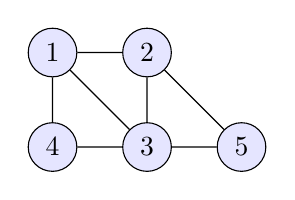
\begin{tikzpicture}[every node/.style={circle,fill=blue!10,draw,minimum size=0.5cm,node distance=1.2cm}]
            \node (1) {$1$};
            \node[right of=1] (2) {$2$};
            \node[below of=2] (3) {$3$};
            \node[left of=3] (4) {$4$};
            \path[draw] (1) -- (2) -- (3) -- (4) -- (1) -- (3);
            \node[right of=3] (5) {$5$};
            \path[draw] (2) -- (5) -- (3);
        \end{tikzpicture}        
    \end{minipage}%   

\end{problem}


\section*{K zamyšlení}


\begin{problem}

    Buď $T=\{(\forall x)(\exists y) S(y)=x,\ S(x)=S(y)\to x=y\}$ teorie v~jazyce $L=\langle S\rangle$ s~rovností, kde $S$ je unární funkční symbol.
    \begin{enumerate}[(a)]
        \item Buď $\mathcal{R}=\langle\mathbb{R},S\rangle$, kde $S(r)=r+1$ pro $r\in\mathbb{R}$. Pro která $r\in\mathbb{R}$ je množina $\{r\}$ definovatelná v~$\mathcal{R}$ z~parametru $0$?
        \item Je teorie $T$ otevřeně axiomatizovatelná? Uveďte zdůvodnění.
        \item Je extenze $T'$ teorie $T$ o~axiom $S(x)=x$ $\omega$-kategorická teorie? Je $T'$ kompletní?
        \item Pro která $0<n\in\mathbb{N}$ existuje $L$-struktura $\mathcal{B}$ velikosti $n$ elementárně ekvivalentní s~$\mathcal{R}$? Existuje spočetná struktura $\mathcal{B}$ elementárně ekvivalentní s~$\mathcal{R}$?
    \end{enumerate}

\end{problem}


% \begin{problem}

%     Známe následující informace o zadávání zakázek:
%     \begin{enumerate}[(i)] \it
%         \item Každý úředník, který je odpovědný za nějakou zakázku a vezme od nějaké společnosti úplatek, je kriminálník.
%         \item Zakázku vyhraje pouze společnost, která podplatí všechny úředníky odpovědné za tuto zakázku.
%         \item Pan Lubor je úředník.
%         \item Nějaká společnost vyhrála nějakou zakázku, za kterou je pan Lubor odpovědný.
%     \end{enumerate}
%     Pomocí rezoluce dokažte, že: {\it (v) Pan Lubor je kriminálník.}
%     \begin{enumerate}[(a)]
%         \item Uvedená tvrzení vyjádřete \underline{sentencemi} $\varphi_1, \dots, \varphi_5$ v jazyce $L=\langle U, Z, S, K, P, V, O, l \rangle$ bez rovnosti, kde $U, Z, S$ a $K$ jsou unární relační symboly a $U(x), Z(x), S(x), K(x)$ znamenají (po řadě) ``$x$ je úředník / zakázka / společnost / kriminálník'', $P, V, O$ jsou binární relační symboly, kde $P(x,y), V(x,y), O(x,y)$ značí (po řadě) ``$x$ podplatil $y$'', ``$x$ vyhrál $y$'' a ``$x$ je odpovědný za $y$'' a $l$ je konstanta označující pana Lubora.
%         \item Pomocí skolemizace předchozích formulí nalezněte otevřenou teorii $T$ (případně ve větším jazyce), která je nesplnitelná, právě když  $\{\varphi_1, \varphi_2, \varphi_3, \varphi_4\} \models \varphi_5$.
%         \item Převedením axiomů $T$ do CNF nalezněte teorii $T'$ ekvivalentní $T$ a axiomatizovanou klauzulemi. Napište $T'$ v množinové reprezentaci.
%         \item Rezolucí dokažte, že $T'$ není splnitelná. Rezoluční zamítnutí znázorněte rezolučním stromem. U každého kroku uveďte použitou unifikaci.
%         \item Nalezněte konjunkci základních instancí axiomů $T'$, která je nesplnitelná.
%     \end{enumerate}

% \end{problem}

\end{document}


